Now that the way the code works is explained, we will show the results of working with the code.
\subsection{visual simulations}
First, we will showcase the visual simulations using a Simulator class object and a BeamSim and SphereSim object.
\subsubsection{Simulator class object}
\begin{figure}[H]
	\centering
	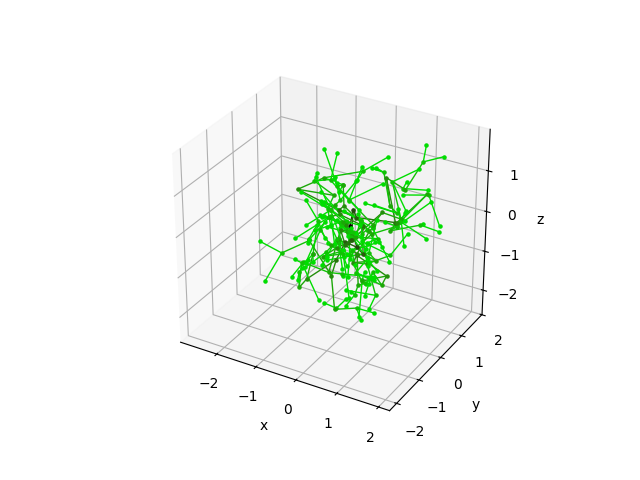
\includegraphics[scale=1]{3D plots/Simulator.png}
	\caption{visual simulation Simulator class object}
\end{figure}
The dots are all green here, because the Simulator class always returns True for \lstinline[language=PythonPlus, style=colorEX]|in_object(x, y, z)|. Note that the center, where the starting point (0, 0, 0) is, contains a lot more darker points, whereas the points towards the edges are predominantly lighter green, signifying later generations.

All visual simulations are taken from the testing code at the bottom of \textit{shapes.py}.
\subsubsection{BeamSim class object}
\begin{figure}[H]
	\centering
	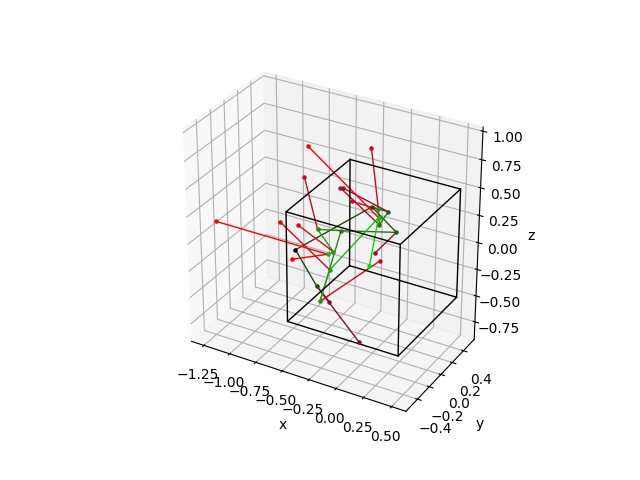
\includegraphics[scale=1]{3D plots/Beam.png}
	\caption{visual simulation BeamSim class object}
\end{figure}
This plot has a mass of 1 and a scale of 1. Thus we get a square. Note that the amount of points is considerably less than the Simulator object. It is also clear that the red points fall outside the volume, while the green lines stay within the mass. Due to the smaller amount of points, it is also considerably easier to follow the order of the points.
\subsubsection{SphereSim class object}
\begin{figure}[H]
	\centering
	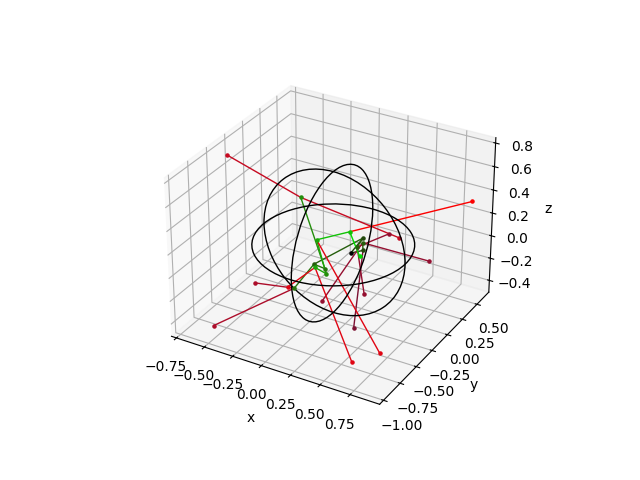
\includegraphics[scale=0.8]{3D plots/Sphere.png}
	\caption{visual simulation SphereSim class object}
\end{figure}
The SphereSim can sometimes be a hard class to get nice plots, as the points sometimes leave the object as soon as the first generation.
\begin{figure}[H]
	\centering
	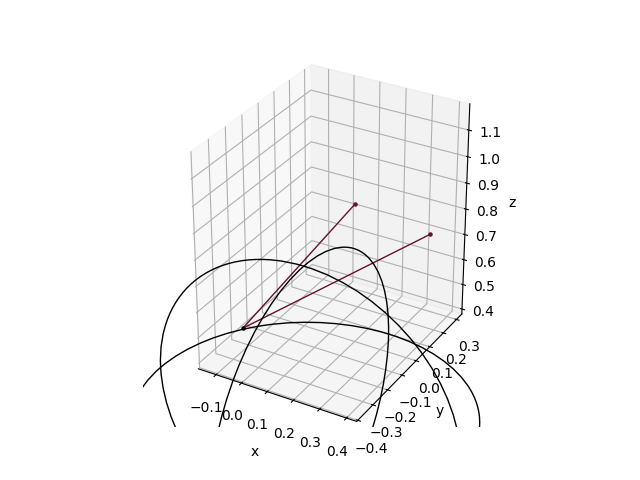
\includegraphics[scale=0.5]{3D plots/Sphere_out_gen1.png}
	\caption{failed visual simulation SphereSim class object}
\end{figure}
\subsection{first task: finding the critical mass of a cube}
The critical mass will be calculated in three steps. First, we will find a general vicinity for the solution by using 100 points to start with. Then we will try this simulation with a smaller range using 1000 simulated points. Finally we will try an even smaller range with 10000 simulated points to estimate a margin of error. All these steps were done multiple times before continuing the code, to make sure the estimates were accurate enough, as the results tend to fluctuate.

For the critical mass of a cube we used scale factor 1 and found a critical mass around a mass of 1.5 with an error margin of 0.3.
\subsection{second task: finding the critical mass of a beam with scale 0.5 and scale 1.5}
For the second task, we used the same methods, but now we used a lot more different scale factors.

We started with a scale of 1.5, for which we found a critical mass of 1 with an error of 0.2.

We then tried a scale of 0.5, but this never seemed to give us a critical mass, even for a mass of 1000. We then experimented with a scale of 2 and 0.9, to get a better understanding of how the critical mass changed depending on the scale. We then found the following data:
\begin{table}[H]
	\centering
	\begin{tabular}{|c|c|}
		\hline
		scale & critical mass \\ \hline\hline
		2 & 0.5 \\ \hdashline
		1.5 & 1 \\ \hdashline
		1 & 1.5 \\ \hdashline
		0.9 & 3 \\ \hdashline
		0.5 & undefined \\ \hline
	\end{tabular}
	\caption{critical mass for different scales}
\end{table}
From this table, we can estimate that it follows an exponential or power curve, but without more points it will be hard to get an accurate fit on the data.
\subsection{third task: finding the critical mass of a sphere}
For the final task, we had to find the critical mass of a sphere. We found that the critical mass was 0.875 with an error margin of 0.125.
\pagebreak